% $Id: solution.tex 
% !TEX root = ../main.tex

\section{Flik: A Bugs Life Debugger}
\label{sec:solution}

The black box behavior of \ac{ML} and \ac{RL} agents posit a problem to understand agents and 
their behavior, specially if unexpected behavior is observed. We posit debuggers as an appropriate 
tool to understand agents' behavior. Moreover, we posit debuggers with the possibility to modify 
programs' state and continue execution using new execution paths are even more appropriate and 
suitable to understand \ac{RL} agents, given their intrinsic nature of continuous interaction with the 
environment. However, currently, there is no debugger for \ac{RL} programs with the desired 
features. The reason for this is that most of the debuggers are postmortem, or do not allow developers
to go back in time to replay and analyze the program state. Additionally, most of the debuggers do not 
allow developers to modify variables. In order to contribute to the development of \ac{RL} programs, 
debugging tools should exhibit the following features:

\begin{description}
    \item[Stepping back:] Due to the execution loop of \ac{RL} programs we 
    want to have a functionality that will allow us to step back the execution to observe the change 
    in state between iterations of the loop. This will let developers interacting directly with the program, 
    without having to stop the execution,  lose the program state, or the training data already 
    accumulated. Such feature will help in identifying the root cause of erroneous agent behavior, 
    whether that is an error in the program's design for particular interactions, or an ill-defined 
    hyperparameter. 
    \item [Modifying variables:] While stepping back into the program's execution, we would want to be 
    able to modify variables' values during the execution. Such feature would help to test out the 
    behavior of an agent with different state-values, or hyperparameters, without having to 
    continuously stop and retrain the agent, which can be very costly and time-consuming. 
\end{description}

These features aim at tackling the problem of interaction with the program, as it allows 
to inspect the behavior of a program with respect to different variable values. Additionally, 
developers may interact with the program execution by going forward and backward, observing the 
effects of specific interactions between the agent and the environment. The capacity to explore the 
execution (backward and forward) would allow for the evaluation of the behavior and quality of 
\ac{RL} programs, helping to improve the development of these programs.

With these features in mind, we present \flik: \textsc{A bugs life}, a back-in-time debugger with the 
possibility to step back in the execution, change values for different variables, and resume execution 
on different execution paths. \flik is not a traditional debugger; it is valuable to debug \ac{RL} 
programs, allowing to evaluate the internal state of the agent, the decisions it makes, and the rewards 
it receives, through the observation of its variables over time. Using the debugger, developers can 
better understand the execution context of \ac{RL} agents in terms of variables, values, environment, 
states and the rewards. 

\flik is a console-based debugger, constructed over the \ac{PDB} debugger. \flik adds features 
such as colored syntax highlighting, tracking of variables' state, and capturing stdout output 
from executed lines of code. The following are the three major features of \flik:
\begin{itemize}
    \item Stores the state in each execution step (\ie action taken by the agent). \flik saves the local 
    and global variables, in a history variable. Additionally, other metadata like the information of the 
    line being executed is saved. This allows us to later step back into specific states in the stored 
    history, and their corresponding location in the code. 
    \item Restores a previous program states as, from the previously stored information, from the 
    stack and heap variables to precisely restore the program's state and its execution context, in 
    order to re-create an alternative execution path. 
    \item Finally, connecting the previous two features, is the action of stepping back. This feature is 
    created as a custom \ac{PDB} command, using the same syntax and form of the native \ac{PDB} 
    commands. The stepping back command takes the state saved at a specific point in the history, 
    and restores the state according to the information at that point --that is, program's state, stack 
    information, and code line. 
\end{itemize}

In Python, the internal state of a program during execution is primarily encapsulated in 
stack frames. Each stack frame contains information about the execution state of a function 
call, including the current line number, local and global variables, and other metadata, as follows:
\begin{itemize}
    \item \scode{f_lineno}: The current line number being executed.
    \item \scode{f_locals}: A dictionary of local variables within the frame.
    \item \scode{f_globals}: A dictionary of global variables accessible within the frame.
    \item \scode{f_code}: A code object representing the function's bytecode and source code metadata.
\end{itemize}

The state is saved in a list that stores snapshots of the frame's state (line and variables) at each 
execution step, which allows stepping back into any state we would want to restore. We use the  
\scode{exec} function that receives the stored \scode{f_globals} and \scode{f_locals} variables as 
parameters. \scode{exec} then executes a list of stored state snapshots (line number 
and local variables) at each step in a specified frame's context (given by the function parameters). 
This allows \flik to simulate running a specific line in the context of a previous frame, maintaining 
both local and global variable references, essentially restoring the saved execution state.

This all done by extending the \ac{PDB} class and adding custom commands to support stepping 
back and a custom interface which allows the user to interact with the debugger. The interface 
displays the code, variables, and execution point, and allows the user (to use the \ac{PDB} 
functions) to pause, step forward, step back, continue or restart the program, as well as to 
modify and inspect variables. 

\fref{fig:debuggerf} shows the general interface of \flik on simple \scode{bubble_sort} function. From 
the top, the first frame (in the blue rectangle Execution frame) we have the running execution, in this 
case the print for the array to be sorted in Line 18 in the second frame. The second frame (in the 
purple rectangle Source code frame) shows the source code that is being debugged. The third frame 
(in the red rectangle Variables frame) shows the variables used in the program so far. Finally, in the 
bottom of the interface we have the interactive console in which developers can send commands to 
\flik to effectively debug the program.

\begin{figure}[h]
    \centering
    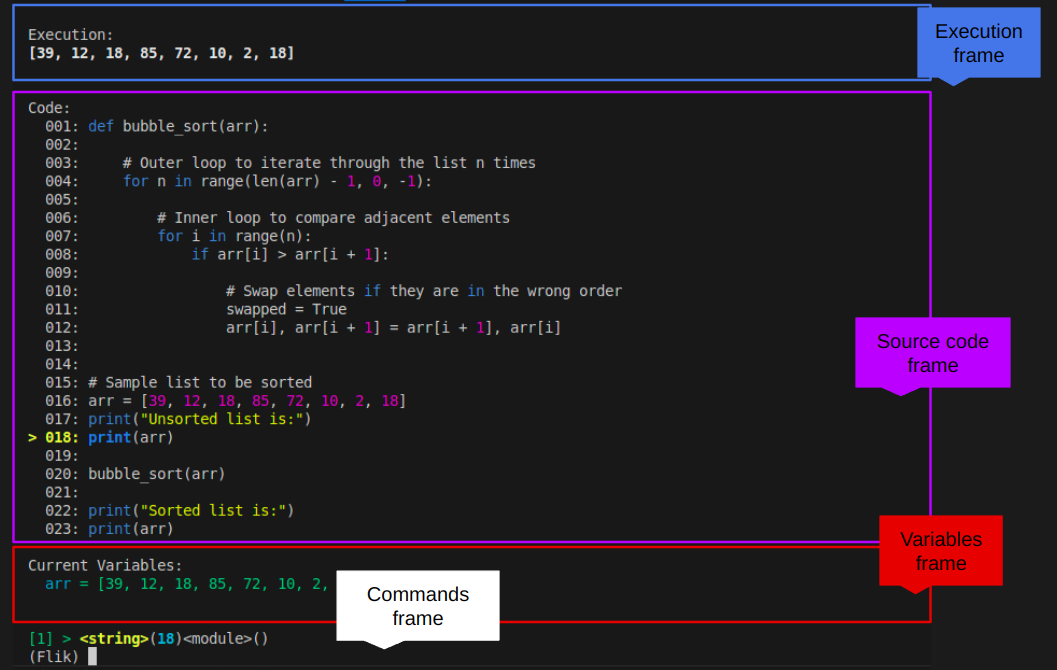
\includegraphics[width=0.9\textwidth]{figures/flik_interface.png}
    \caption{Debugger tool}
    \label{fig:debuggerf}
\end{figure}

% Add example of use step by step. Explain the videos.
We now use a running example to present the features, commands and inner work of \flik. Four 
our running example we use the gridworld \ac{RL} benchmark. The environment consists of a 
$10 \times 10$ grid, shown in \fref{fig:gridworld}. The agent can move in four directions: up, down, 
left, and right at every gridworld cell. However, the movement is not successful in bordering cells 
or cells adjacent to walls (\ie gray-out cells), as it collides with the walls and bounces back to the 
starting position.
There are two kind of rewards that the agent can get, a positive reward of 1 when 
the agent gets to the goal, and a negative reward of -1 when the agent goes to the 
trap. The agent starts in the blue box shown \fref{fig:gridworld}. Now, in the following
example let's say we define our program properly, but we define the $\epsilon$ value 
so small that the agent will not explore the grid, and will not learn properly. 
This will mean that only the first action taken by the agent will be random and after that
with a major probability it will keep only choosing the same action. We can think about 
the worst case scenario, in which the agent will move right and then in the next step it 
will move left, and it will keep doing this for a long time, with a low probability of 
choosing another action. We can use \flik to debug this problem, we can go step by step
inspecting the variables and the actions taken and we can identify specifically that for 
the first state in each episode the agent is taking the same action. We can then go back and
reproduce this problem as many times as we want, and we can change the value of $\epsilon$
to a higher value, so the agent can explore the grid properly. And finish the execution.
This example is shown in the following video: \url{https://drive.google.com/file/d/1NyipuWsRr6ZrIbtlvU5qyooHS2aVsWXc/view?usp=sharing}.



\endinput

